\documentclass[11pt]{article}

\usepackage[T1]{fontenc}
\usepackage[spanish]{babel}
\usepackage{lmodern}
\usepackage[textheight=23cm,headsep=1cm]{geometry}
\usepackage{graphicx}
\usepackage[utf8]{inputenc}
\usepackage{hyperref}
\hypersetup{colorlinks,linkcolor=blue}

\parskip=4mm


\begin{document}

%portada

\begin{titlepage}
    \begin{ttfamily}
        \begin{center}
            \vspace*{1in}
            {\LARGE drManhattan - Manual de usuario}
            \par
            \vspace{0.5in}
            
\includegraphics[width=4.5cm]{imagenes/portada}

            \vspace{0.5in}
            {\large Manuel Pando Muñoz}
            \par
            Proyecto fin de carrera
            \par
            Universidad de Cantabria
            \par
            \vspace{0.5in}
            \today
        \end{center}
    \end{ttfamily}

    \vfill

    \begin{abstract}
        El siguiente documento representa el manual de usuario para la aplicación drManhattan.
    \end{abstract}
\end{titlepage}



\cleardoublepage

\tableofcontents


\newpage

\section{Descripción}
\label{sec:descripcion}

drManhattan nace con motivo del proyecto de fin de carrera de Manuel Pando Muñoz, ofertado por Pablo Sánchez Barreiro en la Universidad de Cantabria para acceder al título de Ingeniero en informática.

El objetivo del proyecto era trata de desarrollar un software que, una vez instalado en los laboratorios con computadores del centro, permitiese controlar el acceso del alumnado a la red durante la realización de pruebas evaluables, de forma que el software permita el uso lícito de la red, pero bloquee el ilícito.

Con uso ilícito nos referimos, por ejemplo, a mirar posibles soluciones en internet, o comunicarse con otro alumno, esto es deseable evitarlo, pero a su vez, el que haya una red que interconecte los computadores permite enviar ficheros de modo casi automático por parte del profesor, o la recogida de los resultados de los alumnos, esos serían usos lícitos.



\newpage

\section{Requisitos}

En la siguiente sección se describen los requisitos necesarios para un uso correcto de drManhattan.

\subsection{Requisitos hardware}

\begin{itemize}

    \item PC Compatible con java.

    \item Memoria RAM de al menos 512MB.

\end{itemize}

La aplicación no hace un uso intensivo de los recursos del sistema, por lo que prácticamente cualquier PC de hoy en día cumple los requisitos.


\subsection{Requisitos software}

\begin{itemize}

    \item Sistema operativo basado en Debian\footnote{\href{http://www.debian.org/misc/children-distros}{Lista de distribuciones basadas en Debian: http://www.debian.org/misc/children-distros}}, de 32 o 64 bits.

    \item Java Runtime Environment 1.6

\end{itemize}

Como se puede observar, la aplicación se ha desarrollado para utilizarse en sistemas Linux.


\newpage

\section{Instalación y desinstalación}

El software drManhattan es distribuido y se compone de dos aplicaciones. Una de ellas es la aplicación utilizada por el profesor y la otra la usada para el alumno.

\subsection{Instalación}

\subsubsection{Visual}

Para simplificar lo más posible la instalación, se han creado archivos .deb diferenciados. Una vez que se tenga decidido qué computador utilizará el profesor y cuales los alumnos, simplemente es hacer doble click en el archivo .deb correspondiente.

\begin{center}

    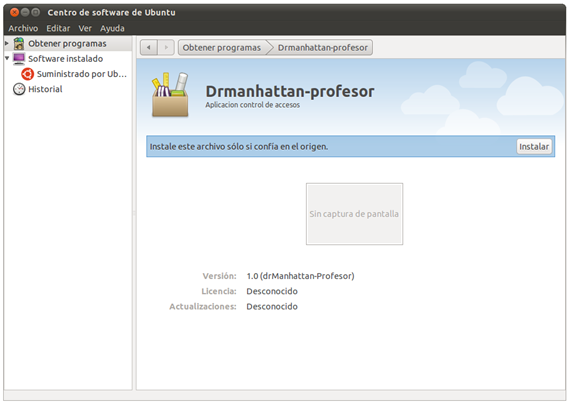
\includegraphics[width=.90\linewidth]{imagenes/inst1}

\end{center}

Tras pulsar el botón de instalar nos pedirá la contraseña de administrador.

\begin{center}

    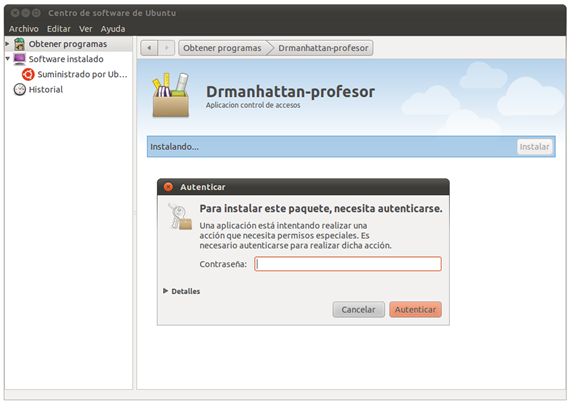
\includegraphics[width=.90\linewidth]{imagenes/inst2}

\end{center}


Después de introducirla vemos como se está instalando.

\begin{center}

    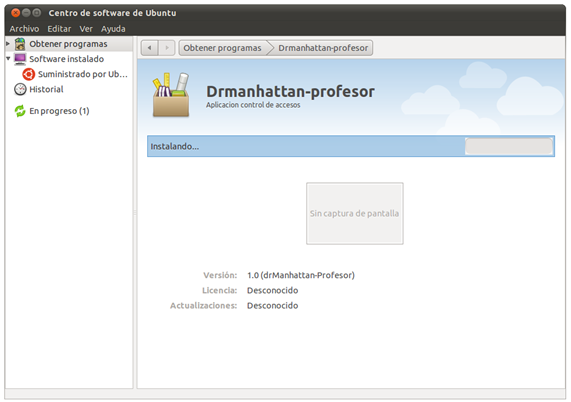
\includegraphics[width=.90\linewidth]{imagenes/inst3}

\end{center}

Al finalizar la instalación, se puede iniciar la aplicación que está ubicada en:

\begin{center}

    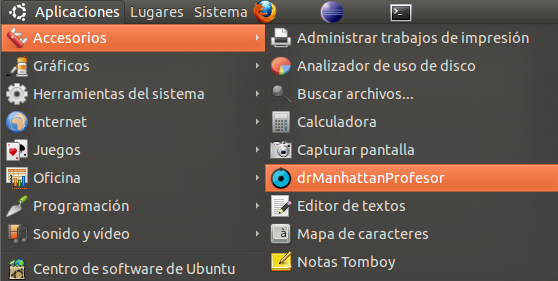
\includegraphics[width=.90\linewidth]{imagenes/inst4}

\end{center}


\subsubsection{Consola}

El proceso de instalación utilizando la consola es el siguiente, también muy simple partiendo de los ficheros .deb.


\begin{center}

    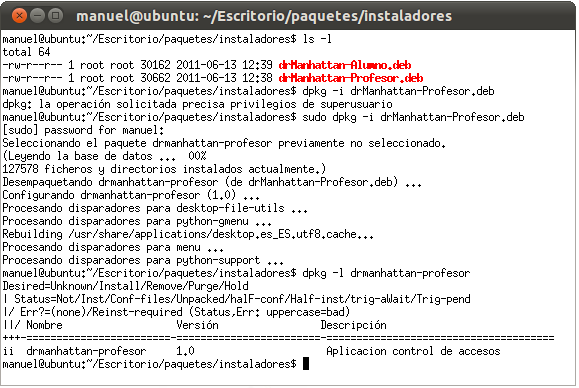
\includegraphics[width=.90\linewidth]{imagenes/instalacionConsola}

\end{center}

Se ejecuta la orden privilegiada dpkg -i paquete.deb y la aplicación queda instalada y lista para usar.

\subsubsection{Compilar código fuente}

Otra opción para utilizar el software es descargarse el código fuente del \href{http://code.google.com/p/drmanhattan/}{repositorio drManhattan en googlecode} y compilarlo localmente. Esto es posible ya que la aplicación utiliza la licencia GPL V3\footnote{\href{http://www.gnu.org/licenses/gpl.html}{Términos de la licencia GPL}}, es decir, es software libre, por lo que se puede descargar el código fuente.




\subsection{Destinstalación}

\subsubsection{Visual}

Para desinstalar el software visualmente, abrir el Centro de software Ubuntu localizado en:

\begin{center}

    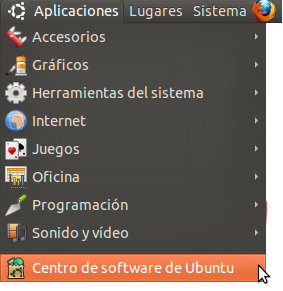
\includegraphics{imagenes/localLizacionCentroSoftware}

\end{center}

Y dentro de el, seleccionar Software Instalado > Otros, aparecerá una lista de paquetes entre ellos los referentes a esta aplicación. Click en desinstalar. Como ocurre en la instalación, también es necesario introducir la contraseña de administrador.

\begin{center}

    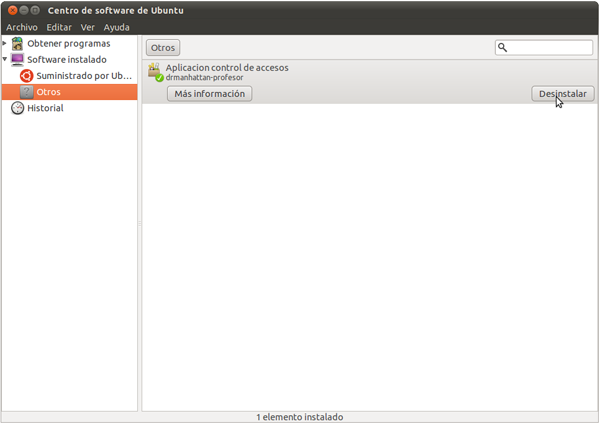
\includegraphics[width=.90\linewidth]{imagenes/desinstalar}

\end{center}

\subsubsection{Consola}

La desinstalación por consola es también muy parecida a la instalación, hay que ejecutar el comando

\begin{center}
    dpkg -P drmanhattan-alumno

    dpkg -P drmanhattan-profesor
\end{center}

En función de cual de los dos paquetes se quiera desinstalar.

\begin{center}

    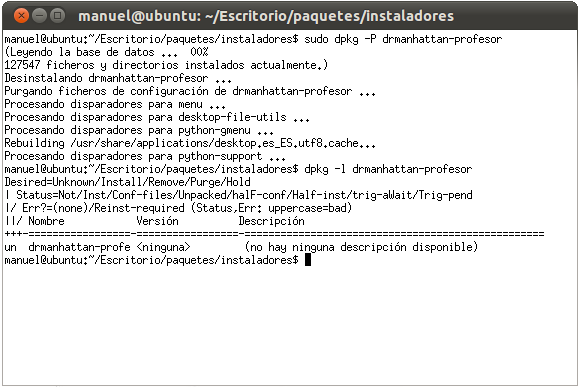
\includegraphics[width=.90\linewidth]{imagenes/desConsola}

\end{center}

Como vemos, tanto la instalación cómo la desinstalación de la aplicación son dos procesos muy sencillos.


\newpage
\section{Aplicación del profesor}

En la siguiente sección se describe la aplicación del profesor, así como las funcionalidades aportadas por ella.

\subsection{Breve explicación de cada componente}

\begin{center}
    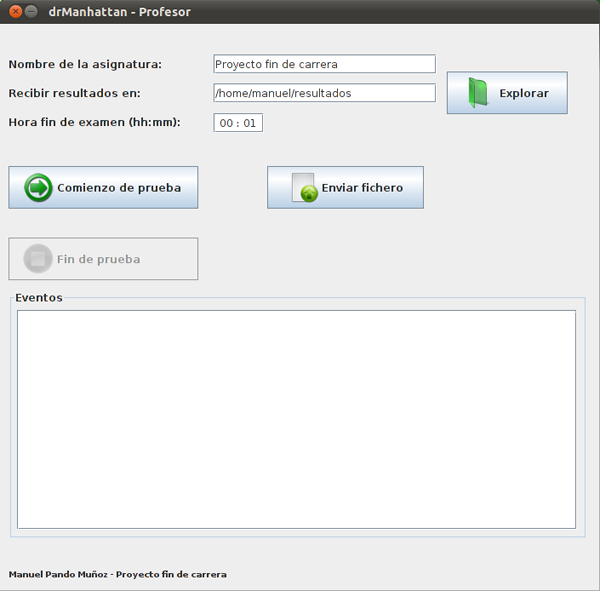
\includegraphics[width=.90\linewidth]{imagenes/GUIProfesor}
\end{center}

En la interfaz tenemos tres campos de texto:
\begin{itemize}
    \item {\bfseries Nombre de la asignatura:} Para definir de que asignatura es la prueba a realizar.
    \item {\bfseries Recibir resultados en:} Para definir, en caso de que los haya, dónde se recibirán los resultados de los alumnos.
    \item {\bfseries Hora fin de examen:} Para definir una hora en la que automáticamente se acabará la prueba.
\end{itemize}

Cuatro botones:

\begin{itemize}
    \item {\bfseries Explorar:} Para escoger cómodamente navegando por el sistema de ficheros un directorio dónde recoger los resultados.
    \item {\bfseries Enviar fichero:} Para escoger un archivo local y enviarlo a los alumnos que realizarán la prueba.
    \item {\bfseries Comienzo de prueba:} Para indicar el comienzo la prueba.
    \item {\bfseries Fin de prueba:} Para indicar la finalización de la prueba.
\end{itemize}

Y una región de texto:

\begin{itemize}
    \item {\bfseries Eventos:} Dónde aparecen en tiempo real mensajes relacionados con la prueba, por ejemplo, la finalización de un alumno.
\end{itemize}

Algunos componentes aparecen deshabilitados, esto es así ya que no tiene sentido finalizar una prueba que no ha empezado todavía. Los componentes se habilitan y deshabilitan dinámicamente durante el transcurso de la prueba según sean o no de utilidad.


\subsection{Enviar fichero de enunciado}

Cuándo los alumnos que realizarán la prueba se han conectado, sección \ref{sec:conectarse}, al pulsar el botón \lq\lq Enviar fichero\rq\rq se abe un diálogo con el que podemos navegar por el sistema de archivos y seleccionar un fichero a enviar.

\begin{center}
    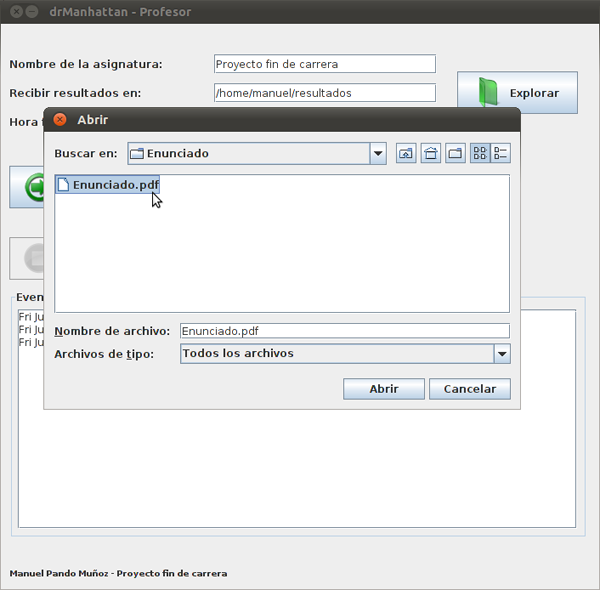
\includegraphics[width=.90\linewidth]{imagenes/enviar}
\end{center}

Cuando finalize el envío se notificará en la región de texto inferior.

\begin{center}
    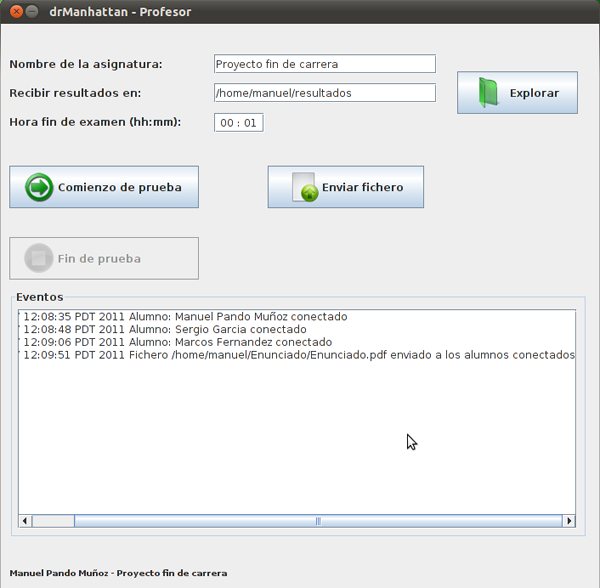
\includegraphics[width=.90\linewidth]{imagenes/eventoEnviar}
\end{center}

Antes del comienzo de la prueba se pueden enviar tantos archivos de enunciado como se desee, con la única limitación de transferirlos de uno en uno.

\subsection{Comienzo de prueba}

Cuándo el docente decide que ha llegado el momento para comenzar la prueba, pulsa el botón \lq\lq Comienzo prueba\rq\rq, esto manda una señal a todos los alumnos conectados y, desde ese momento, dejan de tener acceso a la red.
Antes de comenzar realiza ciertas comprobaciones, entre ellas si se tienen permisos de escritura en el directorio escogido para recibir los resultados, en caso de que no los tuviese, se informa de ello mediante un diálogo modal.

\begin{center}
    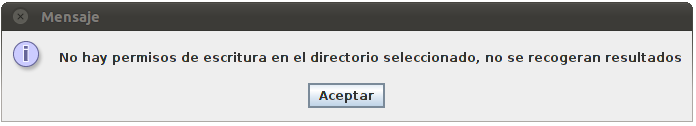
\includegraphics[width=.90\linewidth]{imagenes/comienzoPermisos}
\end{center}

Antes de comenzar definitivamente la prueba, se pide confirmación para evitar posibles errores.




\subsubsection{Pruebas temporizadas}

El software drManhattan ofrece la posibilidad de definir una hora límite para la duración de la prueba, mediante el campo de texto \lq\lq Hora fin de examen\rq\rq. Cuándo comienza una prueba, se calcula el límite de tiempo y se notifica a las aplicaciones de los alumnos conectadas. Si se introduce una hora inferior a la actual se obvia y la prueba no tiene duración prefijada. El tiempo restante aparecerá en la interfaz del alumno a modo de cuenta atrás, produciendo un aviso cuando resten 5 minutos para la finalización automática.

\begin{center}
    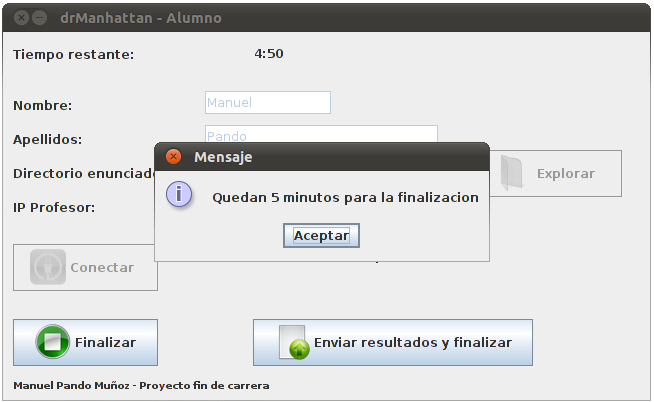
\includegraphics[width=.90\linewidth]{imagenes/tiempoLimite}
\end{center}


\subsection{Finalización de prueba}
\label{sec:finalizacionPrueba}

Las pruebas pueden finalizar de cuatro modos distintos:

\begin{enumerate}

    \item Finaliza el profesor manualmente.

    \item Finaliza por tiempo automáticamente.

    \item Finaliza el alumno sin entregar resultados.

    \item Finaliza el alumno entregando resultados.

\end{enumerate}

La primera ocurre cuándo el profesor pulsa el botón de \lq\lq Fin de prueba\rq\rq, esto manda una señal a las aplicaciones de los alumnos indicando que se ha acabado el tiempo, no se recogerán resultados después de pulsar el botón.

La segunda sucede durante una prueba temporizada, cuándo se agota el tiempo destinado para la misma. Tampoco se recogen resultados después de que acabe la prueba.

La tercera se explica en la sección \ref{sec:finAlumno} y la cuarta en la \ref{sec:finResultados}.

\subsubsection{Recogida de resultados}

Cuándo los alumnos envían sus resultados, la aplicación del profesor los recoge y crea un árbol de directorios tomando cómo base el establecido en el campo de texto \lq\lq Recibir resultados en\rq\rq. Dentro de ese directorio se crea otro con el nombre de la asignatura definido y a su vez, dentro de el, se crea, por cada alumno que envíe resultados, otra carpeta utilizando los apellidos y el nombre del alumno, dónde se almacena el archivo de resultados.

Se realiza una comprobación de integridad del fichero utilizando el algoritmo MD5 para garantizar la falta de errores durante la transferencia.

\newpage
\section{Aplicación del alumno}

En la siguiente sección se describe la aplicación del alumno, así como las funcionalidades aportadas por ella.

\begin{center}
    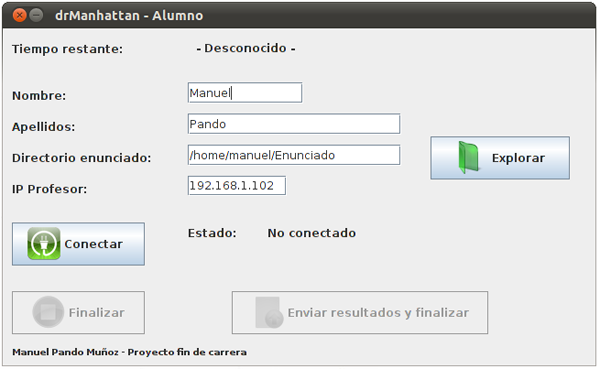
\includegraphics[width=.90\linewidth]{imagenes/GUIAlumno}
\end{center}


\subsection{Breve explicación de cada componente}

En la interfaz del alumno tenemos lo siguiente:

Cuatro campos de texto:

\begin{itemize}

    \item {\bfseries Nombre:} Para definir el nombre del alumno que realizará la prueba
    \item {\bfseries Apellidos:} Para definir los apellidos del alumno que realizará la prueba
    \item {\bfseries Directorio enunciado:} Para definir, en caso de que los haya, dónde se recibirán los archivos de enunciado.
    \item {\bfseries IP profesor:} Para definir el equipo del profesor, al que se conectará la aplicación.

\end{itemize}

Cuatro botones

\begin{itemize}

    \item {\bfseries Explorar:} Para escoger cómodamente navegando por el sistema de ficheros un directorio dónde recoger el enunciado.
    \item {\bfseries Conectar:} Conectarse a la aplicación del profesor.
    \item {\bfseries Finalizar:} Finalizar la prueba sin enviar resultados.
    \item {\bfseries Enviar resultados y finalizar:} Escoger un único fichero cómo resultado, enviarlo al profesor y finalizar la prueba.

\end{itemize}

Y dos etiquetas dinámicas:

\begin{itemize}

    \item {\bfseries Tiempo restante:} Muestra el tiempo restante para la finalización de la prueba en caso de estar temporizada.

    \item {\bfseries Estado: } Muestra el estado en el que se encuentra la aplicación, No conectado, Realizando prueba, Transfiriendo fichero...

\end{itemize}

Del mismo modo que en la interfaz del profesor, los componentes se habilitan o no en función de su utilidad durante la prueba.

\subsection{Conectarse}
\label{sec:conectarse}

Al pulsar el botón \lq\lq Conectar\rq\rq, se realizan comprobaciones a los valores de los campos de texto introducidos, similares a las comprobaciones que se ejecutan en la aplicación del profesor al comenzar una prueba. Si está todo correcto la aplicación conectará con la del profesor. Se puedo comprobar ya que la etiqueta Estado cambia su valor.

\begin{center}
    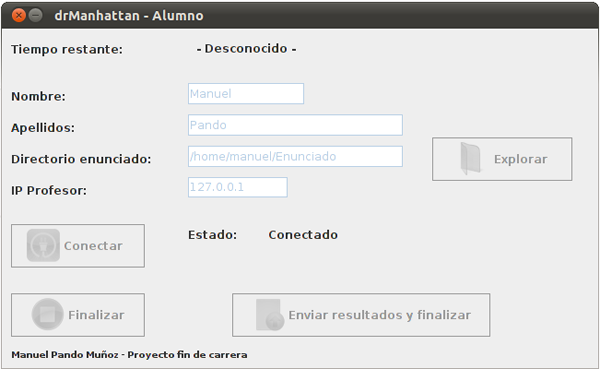
\includegraphics[width=.90\linewidth]{imagenes/Conectado}
\end{center}

\subsection{Finalización de prueba}
\label{sec:finAlumno}

Cómo comentamos en la sección \ref{sec:finalizacionPrueba} el alumno puede finalizar la prueba enviando o no resultados.

Para finalizar la prueba sin enviar resultados basta con pulsar el botón \lq\lq Finalizar\rq\rq, preguntará si estamos seguros y finalizará la prueba, permitiendo de nuevo el acceso a la red. Una vez que se finaliza, no se puede volver a conectar.

\subsubsection{Envío de resultados}
\label{sec:finResultados}

En el caso de que se deseen enviar resultados se utilizará el botón \lq\lq Enviar resultados y finalizar\rq\rq. Hay que tener en cuenta que sólo es posible mandar un único fichero de resultados, por lo tanto, si se tienen varios, hay que empaquetarlos de algún modo, un fichero .tar, por ejemplo.

\begin{center}
    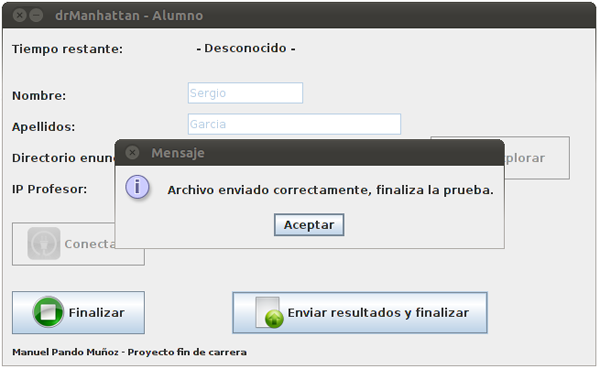
\includegraphics[width=.90\linewidth]{imagenes/finResCorrecto}
\end{center}

Si hay algún problema en el envío del fichero, se notifica, tanto al alumno como al profesor, para que lo recoja de otro modo.


\newpage
\section{Protección frente a errores en el sistema}

El software drManhattan, concretamente en la parte del alumno, es capaz de guardar su estado, es decir, si durante la realización de una prueba, algún alumno, por el motivo que sea, se ve obligado a reiniciar el sistema, cuando se vuelva a iniciar la aplicación, esta reconectará de forma automática con la aplicación del profesor, volviendo al estado previo, antes del error.

\end{document} 